
\subsection{Product perspective }

\emph{myTaxiService} (TS) software can be decomposed into four different
interacting subsystems (Figure 1):
\begin{enumerate}
\item the \emph{passenger web application} (PWA): it's a web portal that
allows passenger to request a taxi, register, login, reserve a taxi
and cancel or modify previous reservations. PWA has to be able to
identify passenger's position using, if available, the browser geolocalization
support.
\item the \emph{passenger mobile application }(PMA): it's an application
that shall be installed on passengers' smartphone performing the same
functions of PWA. PMA needs also to communicate to a GPS application
within the mobile phone, if any available, to retrieve the passenger's
position.
\item the \emph{taxi driver mobile application} (TMA): it's an application
that shall be installed on taxi drivers' smartphone in order to allow
them to receive requests coming from the system, decide to confirm
or reject requests and inform the system about their availability. 
\item the \emph{queue management system} (QMS): it's a software aimed to
compute realtime the distribution of the taxis in the city interfacing
with the GPS system of each taxi, decide which taxi assign to a request
and send to taxi drivers several notifications.
\end{enumerate}
TS has also to be integrated with the previous taxi management system
based on phone calls in order to allow call center operators to forward
requests, therefore a specific interface shall be designed. Moreover,
the system has to be provided with specific interfaces and APIs in
order to allow future requirements extensions.

\begin{figure}
\begin{centering}
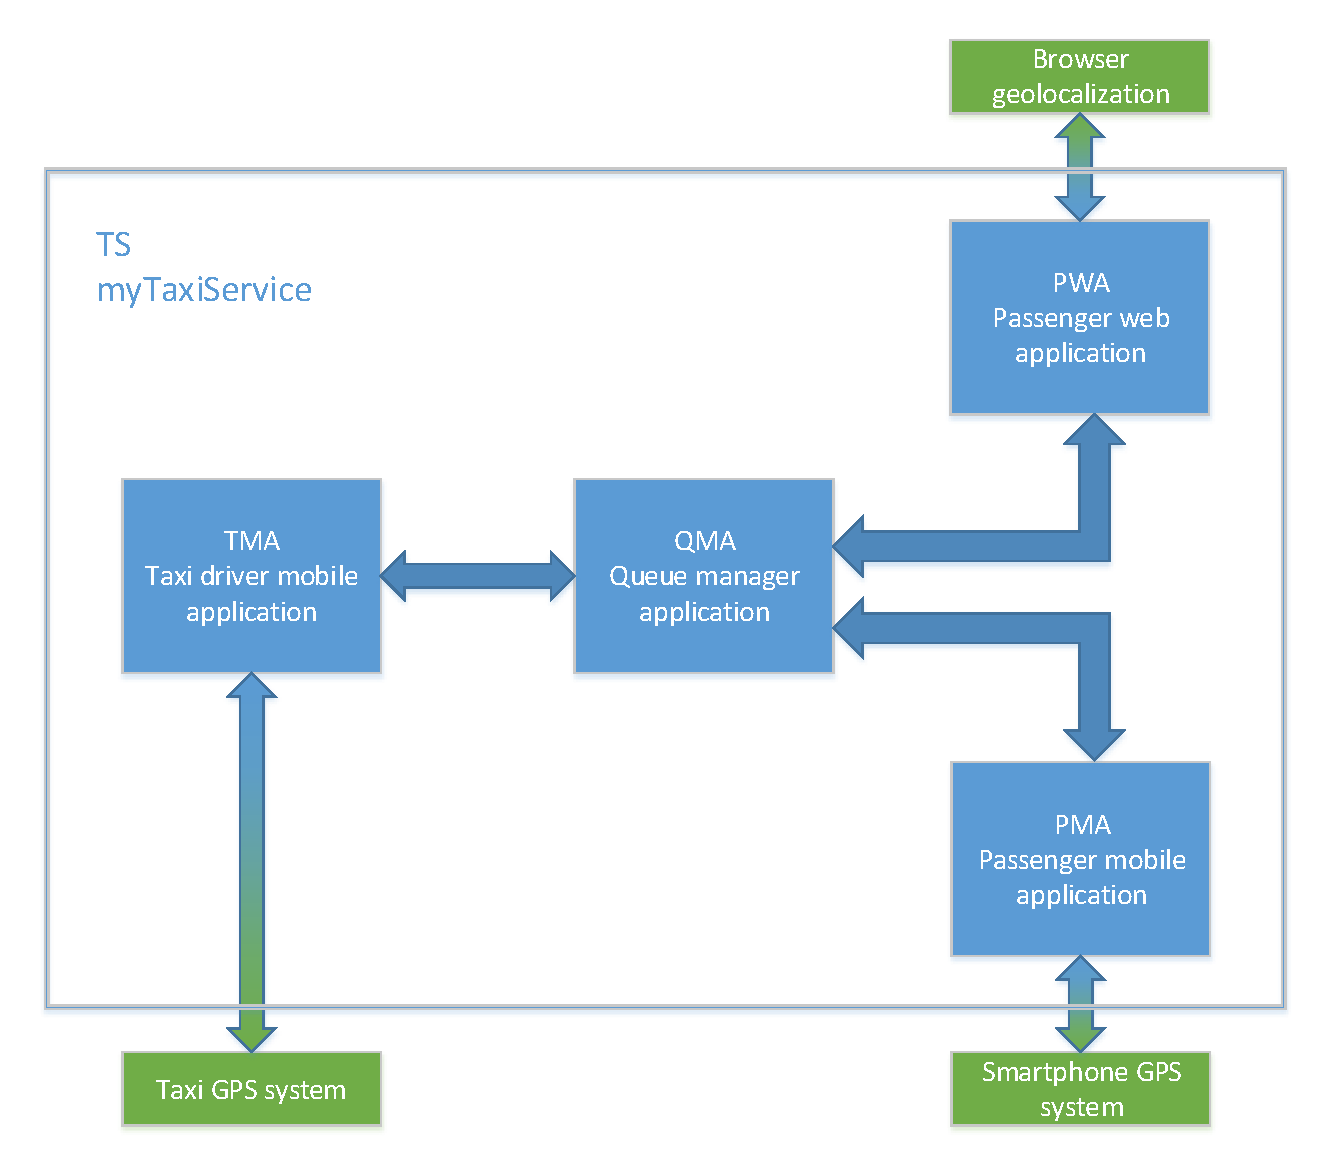
\includegraphics[scale=0.5]{overall-description/Diagram}
\par\end{centering}

\protect\caption{Block schema representing the conceptual interaction between subsystems.}


\end{figure}



\subsection{User characteristics}

Main addressee of myTaxiService are passengers and taxi drivers. Users
are not expected to have specific knowledge or technical expertise
but it is assumed they are able to operate the internet and to have
access to it.


\subsection{Constraints }


\subsubsection{Regulatory policies}

The following regulatory policies has to be met by the software.
\begin{itemize}
\item Since user's geographic position needs to be shared within the application
(either PMA or PWA) to ensure the expected behavior of the system,
users has to agree in advance to specific terms and conditions. 
\item Taxi drivers are obliged not to spread possible collected information
about passengers.
\end{itemize}

\subsubsection{Hardware limitations }

The following hardware limitations has to be met.
\begin{itemize}
\item Mobile passengers has to download the free application from the store
(PlayStore for Android users, AppStore for iPhone users, Windows store
for Windows users). It is assumed that the mobile phones have enough
primary memory to run the application.
\item The browser used by web passengers to access the system must have
cookies enabled.
\item Each taxi driver is provided with a smartphone and the application
TMA must be installed.
\end{itemize}

\subsection{Domain assumptions}

Considering the specific application domain and according to the information
provided by stakeholders we can assume that the following assertions
are always valid.
\begin{lyxlist}{00.00.0000}
\item [{{[}D1{]}}] A taxi driver always executes indications communicated
by the system (e.g. move notifications), except in case of emergency.
\item [{{[}D2{]}}] Each taxi is provided with a GPS system. If GPS system
is not available taxi is considered out of service.
\item [{{[}D3{]}}] A taxi can be stopped along the road by a passenger
if and only if it is waiting without passenger or moving but not for
carrying out a request. In this case taxi driver informs the system
about his/her unavailability.
\item [{{[}D4{]}}] When a taxi driver finishes to carry out a request he/she
informs the system about his availability.
\item [{{[}D5{]}}] When a taxi driver starts his work-shift sets his/her
state from out of service to available.
\item [{{[}D6{]}}] When a taxi driver ends his work-shift if the current
state is available then the taxi state becomes out of service; otherwise
taxi driver finishes to carry out the current request and after that
the taxi becomes out of service.
\item [{{[}D7{]}}] When a taxi driver gets to the meeting place, waits
for 10 minutes; if passenger does not arrive taxi driver informs the
system.
\item [{{[}D8{]}}] A taxi is assigned to a unique taxi driver at time.
It is possible that some taxi drivers are not assigned to any taxi
or vice versa.
\item [{{[}D9{]}}] If a ride gets out of the city the taxi driver comes
back to the last zone before informing TS of his availability.
\item [{{[}D10{]}}] There are only two types of taxi: normal (4 seats)
and minivan (9 seats).
\item [{{[}D11{]}}] Each available taxi belongs to exactly one queue at
time. Busy or out of service taxis do not belong to any queue.
\item [{{[}D12{]}}] TS is available only in the city, no requests coming
from outside of the city boundary are accepted.
\item [{{[}D13{]}}] Taxi drivers have always access to the Internet.
\item [{{[}D14{]}}] Taxi drivers' work-shifts are managed in order to ensure
that at each moment the number of in service taxis is at least 50\%
of the total number of taxis.
\item [{{[}D15{]}}] Taxi drivers go in emergency state only in case of
car accident or similar events.
\item [{{[}D16{]}}] Taxi can move without limitations inside the zone assigned
by TS system but they cannot change the zone without a notification
from the system.
\end{lyxlist}
Note that also taxi drivers are identified by the system but registration
of the taxi driver is not part of the TS system since it reasonably
involves contractual issues (taxi driver has to make an agreement
with the company) that cannot be directly managed by the system. Therefore
registration is not performed by taxi driver.


\subsection{Possible future extensions}

The following are reasonable possible future extensions to the TS
system; they are mainly meant to further improve the usability and
the performances of the service. They will not be discussed in details.
\begin{itemize}
\item At present, queues has a fixed suitable number of available taxis
which is supposed to be calculated using previous data about the number
of requests coming from each zone. However the distribution of the
requests can vary not only \emph{spatially} (from one zone to an other)
but also \emph{temporally} (for each zone at different moments of
the day the number of requests might be different). Also in different
days of the week the distribution of requests may vary significantly.
A possible solution to make TS more adaptive is the one in which the
suitable number of taxis for each queue is periodically determined
integrating data collected from the requests in a certain time horizon
(for instance once a week).
\item At the moment TS system does not handle payments, since users are
expected to pay the ride cash or with credit card to the taxi driver;
online payments can be implemented within TS system. Both PWA and
PMA should allow registered users to pay the price of the ride using
credit card or paypal; cash payment should be still possible.
\item At the moment, passenger requesting a taxi can only see the estimated
waiting time and the code of the taxi, while visualizing also the
current position of the incoming taxi should be more useful.
\item An evaluation system of the quality of service can be added, allowing
passengers to express an opinion about taxis.\end{itemize}

